\documentclass[11pt,a4paper]{article}
\usepackage[utf8]{inputenc}
\usepackage[spanish]{babel}
\usepackage{amsmath}
\usepackage{amsfonts}
\usepackage{amssymb}
\usepackage{graphicx}
\usepackage{float}
\usepackage{caption}
\captionsetup[table]{name=Tabla}
\setlength{\parindent}{0pt}
\usepackage[left=2cm,right=2cm,top=2cm,bottom=2cm]{geometry}
\author{Marina Esgueva Ruiz}
\begin{document}
\section{Experimentación numérica}
La calidad de las soluciones aproximadas obtenidas con el método de las RBF depende fuertemente de diversos parámetros que influyen en el mismo. Algunos de estos parámetros son la colocación y el número de centros, el tipo de RBF utilizadas como funciones básicas y el parámtro de forma de dichas funciones. Para medir la calidad de las aproximaciones calculadas se utiliza el error cuadrático medio, denotado por ECM, que se calcula de la siguiente forma: 
$$ECM=\sqrt{\frac{1}{M}\sum_{i=1}^M (f(x_i)-s(x_i))^2}$$
donde, \\
$x_1,\ldots,x_m$ son puntos distribuidos en una rejilla uniforme en el dominio, \\
$u$ es la solución real de la EDP,\\
$s$ es la solución aproximada de la EDP. 
Los primeros experimentos numéricos se lleva a cabo suponiendo conocida la solución real de la EDP. Sin embargo, en la práctica, no es posible conocer la solución de la EDP por lo que más adelante se definirá una estimación del error que pueda ser calculada sin más información que la ecuación y sus condiciones de frontera. \\
Durante la experimentación numérica trabajamos con las siguientes EDP con dominio en el cuadrado unidad $\Omega$: 
\begin{equation}
\left \lbrace \begin{array}{cc}
\ \Delta u(x,y)=-\dfrac{5}{4}sin(\pi x) cos(\frac{\pi y}{2}), & (x,y) \in \Omega \\
\ u(x,y)=sin(\pi x), & (x,y)\in \Gamma_1, \\
\ u(x,y)=0, & (x,y) \in \Gamma_2\\ 
\end{array} \right.
\label{edp1}
\end{equation}
donde $\Gamma_1=\lbrace (x,y):0\leq x \leq 1, y=0 \rbrace$ y $\Gamma_2= \partial \Omega \backslash \Gamma_1$.\\
Se puede verificar fácilmente que la solución de la ecuación es: 
$$u(x,y)=sin(\pi x) cos(\frac{\pi y}{2}).$$
\begin{figure}[H]
\centering
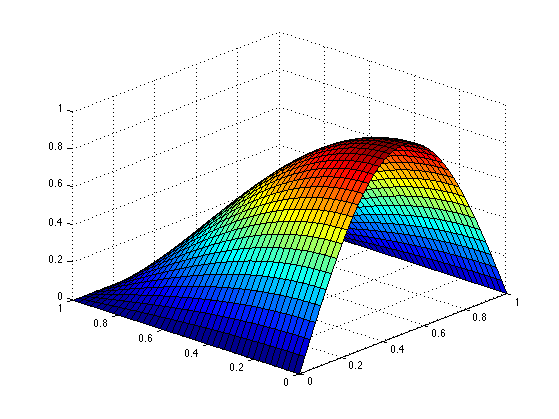
\includegraphics[scale=.5]{u1.png}
\caption{Solución de EDP $(\ref{edp1})$}
\end{figure}
\begin{equation}
\left \lbrace \begin{array}{cc}
\ \Delta u(x,y)=8e^{2x+2y}, & (x,y) \in \Omega\backslash \partial \Omega \\
\ u(x,y)=e^{2x+2y}, & (x,y)\in \partial \Omega, \\
\end{array} \right.
\label{edp 2}
\end{equation}
Es fácil ver que la solución de la ecuación es $e^{2x+2y}$. 
\begin{figure}[H]
\centering
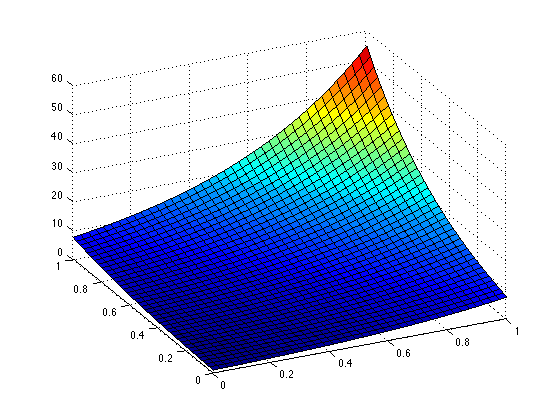
\includegraphics[scale=.5]{u3.png}
\caption{Solución de la EDP $(\ref{edp 2})$}
\end{figure}
\subsection{Distribución y número de centros}
En los primeros experimentos llevados a cabo se trabaja con un parámetro de forma fijo y variamos el número de centros. Además se diferencia entre colocar todos los centros dentro del dominio, o desplazar los centros de la frontera ligeramente fuera del dominio. Para cada una de las aprocimaciones obtenidas se recoge el error cometido en la paroximación así como el condicionamiento de la matriz de colocación utilizada. Los centros los distribuimos en una rejilla uniforme en el dominio: 
\begin{figure}[H]
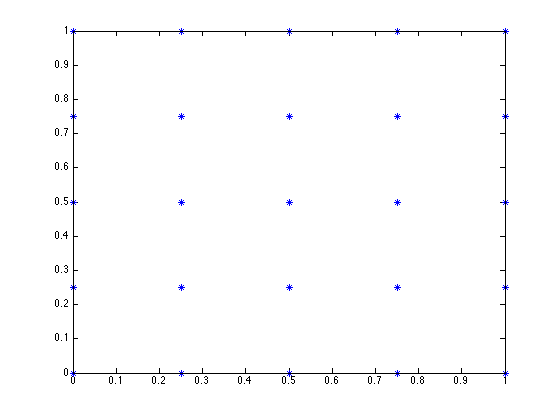
\includegraphics[scale=.45]{distribucion1}
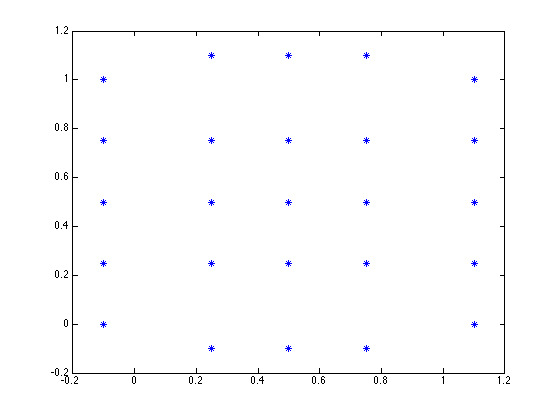
\includegraphics[scale=.45]{distribucion2}
\caption{Distribución de los centros. A la izquierda, todos los centros en el dominio y a la derecha, algunos centros deslplazados fuera del dominio. }
\end{figure} 
\begin{table}[H]
\centering
\caption{Inversas ulticuádricas. $\epsilon=3$. Puntos de colocación distribuidos uniformemente.}
\begin{tabular}{|c|cc|cc|}
\hline
\ & \multicolumn{2}{|c|}{Centros en la frontera} & \multicolumn{2}{|c|}{Centros fuera del dominio} \\
\hline
\ $N$& ECM & Condicionamiento & ECM & Condicionamiento \\
\hline
\ 9 & 1.55e-01 & 5.55e+01& 1.68e-01 & 6.01e+01 \\
\ 25 &  3.41e-02& 5.76e+02 & 2.40e-02 &6.18e+02  \\
\ 81 & 5.73e-03 & 1.50e+05&  3.28e-03 & 1.27e+05 \\
\ 169 & 1.47e-03 &3.46e+07  & 8.29e-04&1.97e+07  \\
\ 289 &4.17e-04  & 7.64e+09&  2.34e-04&2.99e+09  \\
\ 1089 & 3.69e-06 & 8.37e+19 &   2.15e-06 &5.97e+18  \\
\hline
\end{tabular}
\label{primera comparacion}
\end{table}
Observamos que aumentar el número de centros mejora la calidad de las soluciones aproximadas. Por el contrario, el condicionamiento de las matrices de colocación aumenta. En todos los casos el error cometido en la aproximación es menor si desplazamos los centros correspondientes a la frontera fuera del dominio. Sin embargo, estas diferencias no son significativas. 
\end{document}